
\usetikzlibrary{positioning}
\tikzset{main node/.style={circle,fill=blue!20,draw,minimum size=1cm,inner sep=0pt},
            }

  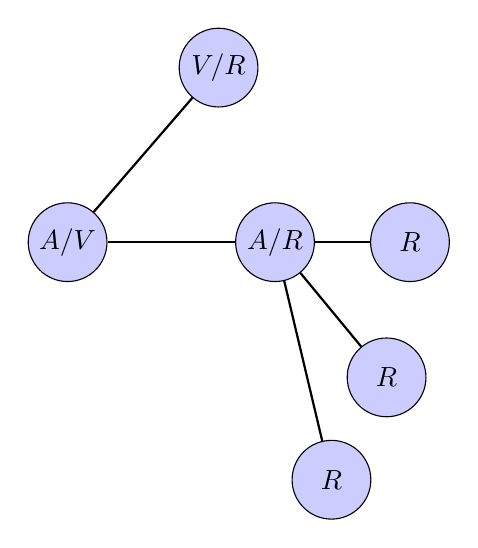
\begin{tikzpicture}
    \node[main node] (1) {$V/R$};
    \node[main node] (2) [below left = 1.5cm and 1.2cm of 1]  {$A/V$};
    \node[main node] (3) [below right = 1.5cm and 0.0cm of 1] {$A/R$};
    \node[main node] (4) [below right = 2.3cm and 0 cm of 3] {$R$};
    \node[main node] (5) [below right = 1cm and 0.7cm of 3] {$R$};
    \node[main node] (6) [right = 0.7cm  of 3] {$R$};

    \path[draw,thick]
    (1) edge node {} (2)
    (2) edge node {} (3)
    (3) edge node {} (4)
    (6) edge node {} (3)
    (5) edge node {} (3);
    %%
    
\end{tikzpicture}
